%************************************************
\chapter{Appendix 3.2: Chapter 3 - Supplementary figures}\label{ch:Appendix3.2}
%************************************************
\renewcommand{\thefigure}{A.3.2.\arabic{figure}}
\setcounter{figure}{0}

\renewcommand{\thetable}{A.3.2.\arabic{table}}
\setcounter{table}{0}

\begin{figure}[ht!]
\centering
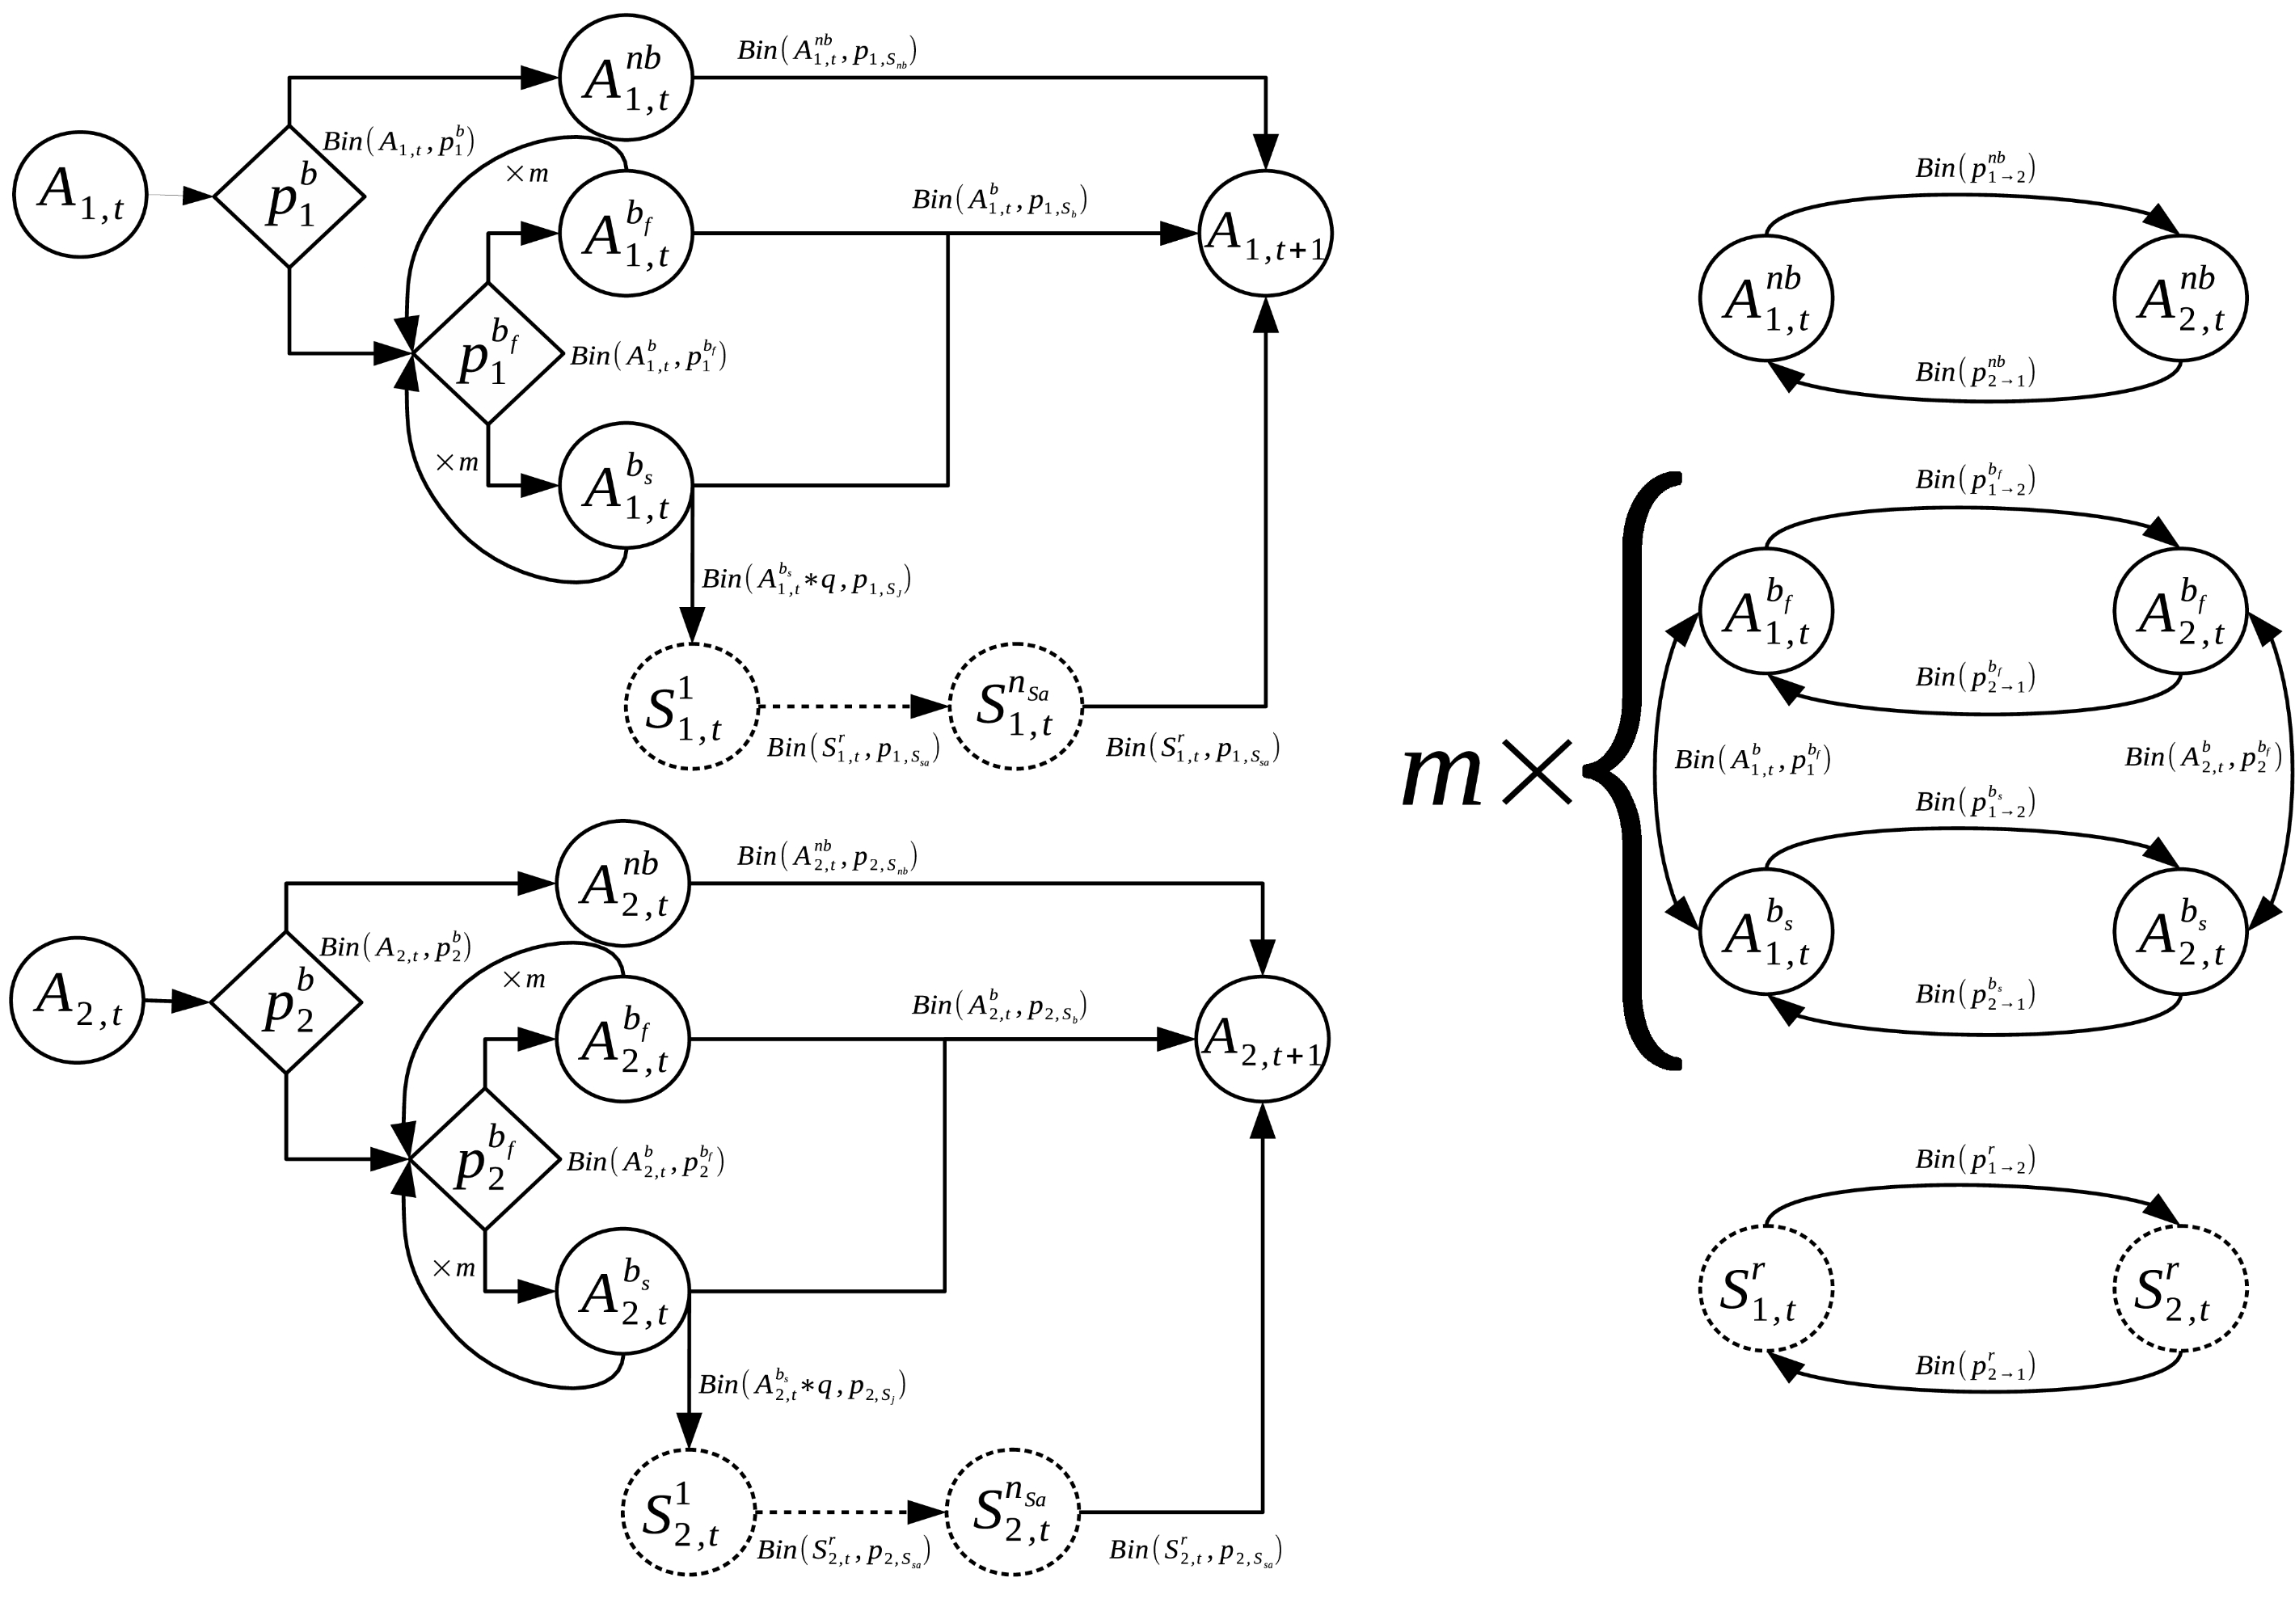
\includegraphics[width=\textwidth]{./Figures/Appendix3_2/Fig_1.jpg}
\caption[Flowchart of the model]{
Flowchart of the stochastic simulation model. Notation is the same as in Table
\ref{tab:tabApp3.1.1} above.}
\label{fig:figApp3.2.1}
\end{figure}

\begin{figure}
\centering
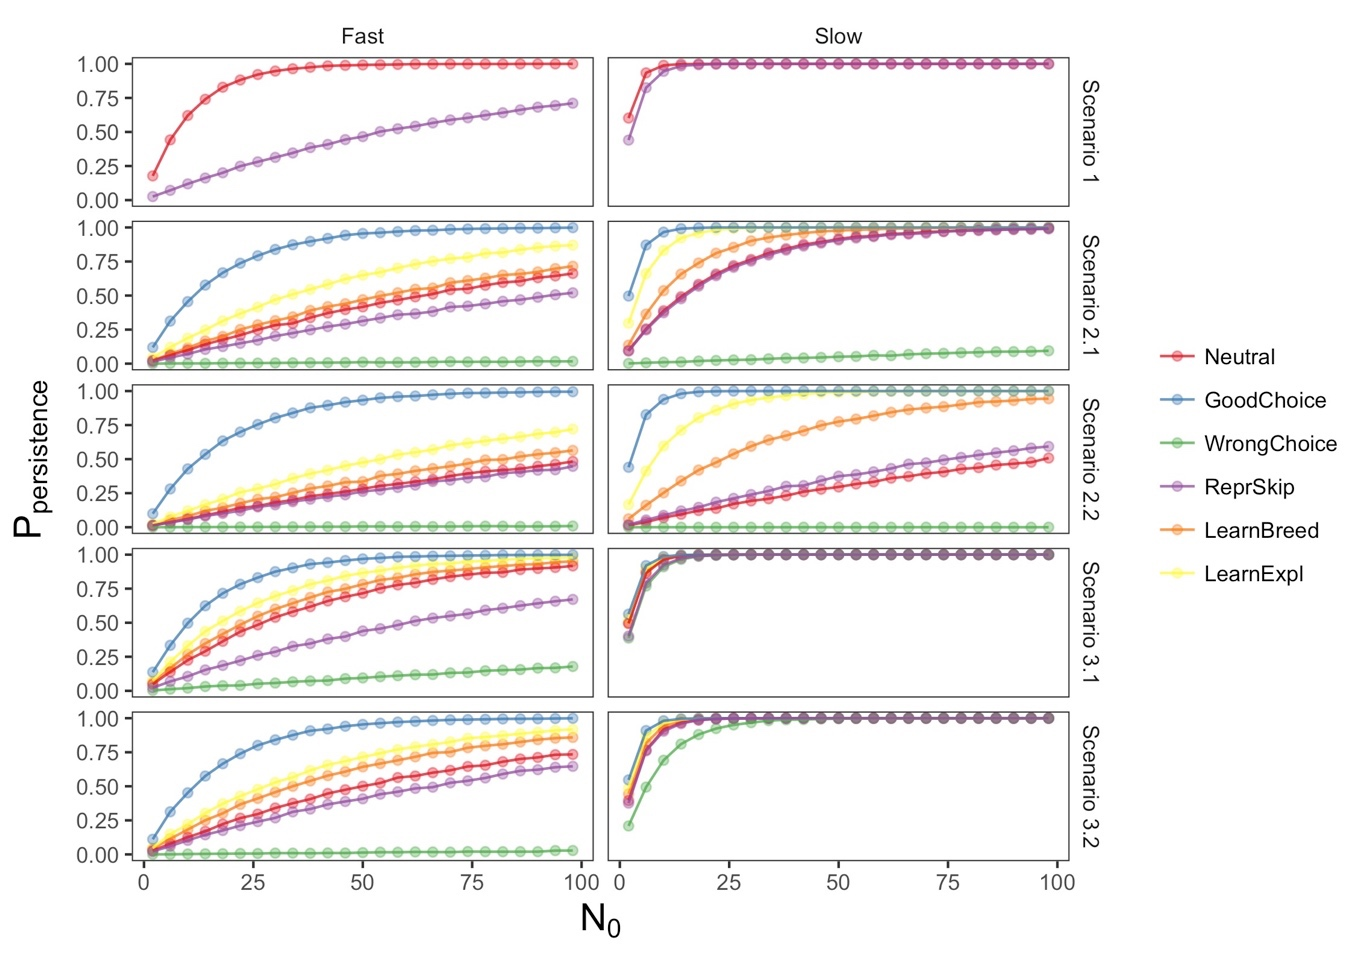
\includegraphics[width=\textwidth]{./Figures/Appendix3_2/Fig_2.jpg}
\caption[Persistence with strong behavioural responses]{
Simulations of probability of population persistence as a function
of behavioural responses for different initial population sizes according to
different life histories (fast and slow). See figure \ref{fig:fig3.1} for
details. In this case we shown the results for simulations with strong
behavioural responses.}
\label{fig:figApp3.2.2}
\end{figure}

\begin{figure}
\centering
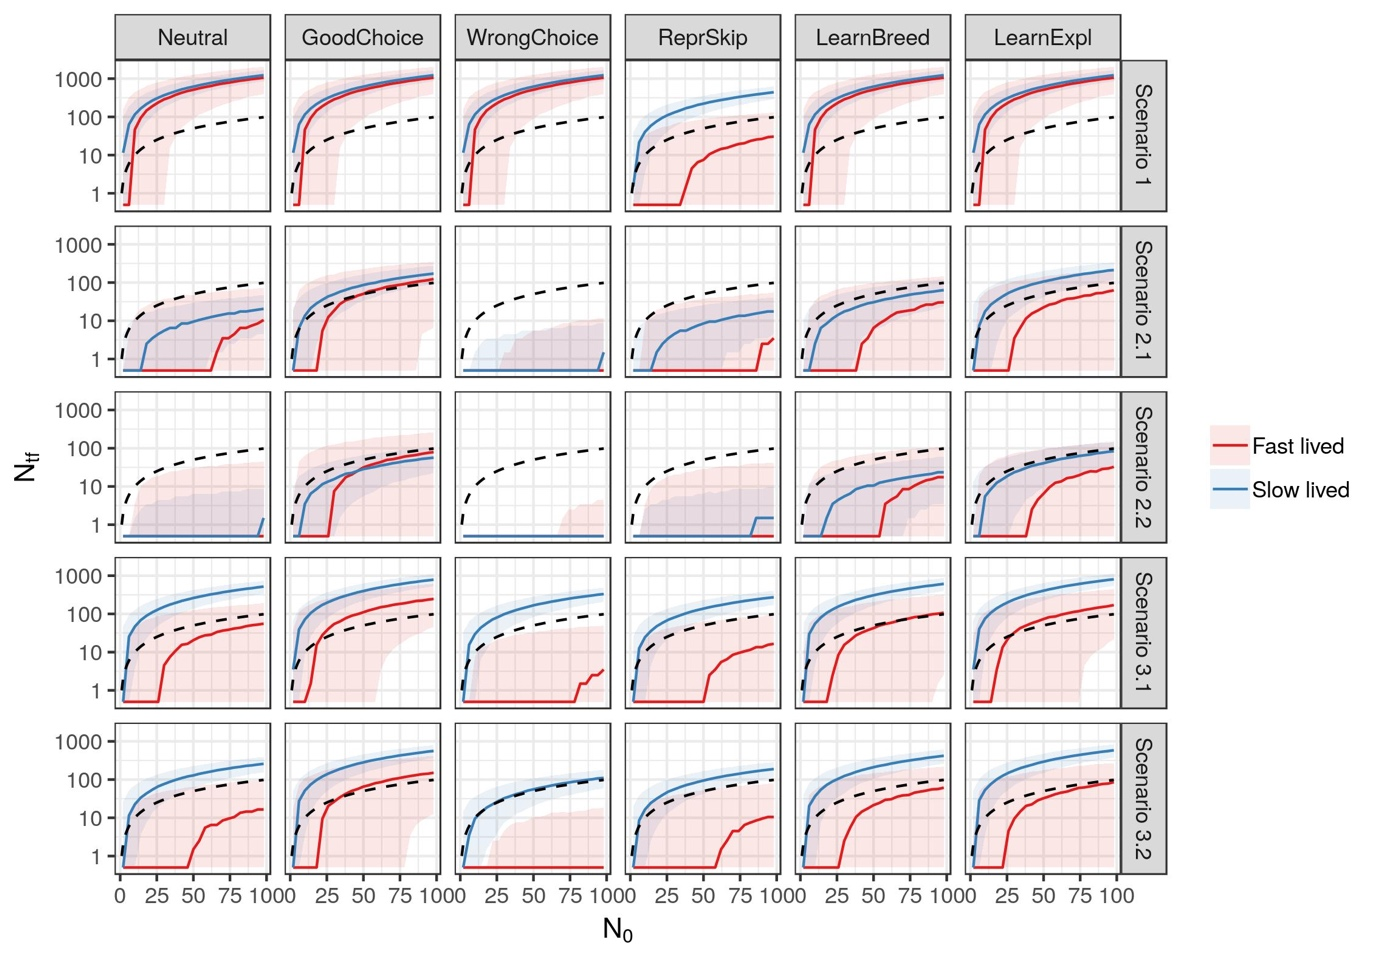
\includegraphics[width=\textwidth]{./Figures/Appendix3_2/Fig_3.jpg}
\caption[Effects on $N_{tf}$]{
Final population size ($N_{tf}$, median and 95\% confidence interval
of the 10000 replicates) of the simulations shown in figure \ref{fig:fig3.1}.
Black dashed lines show the initial population size.}
\label{fig:figApp3.2.3}
\end{figure}

\begin{figure}
\centering
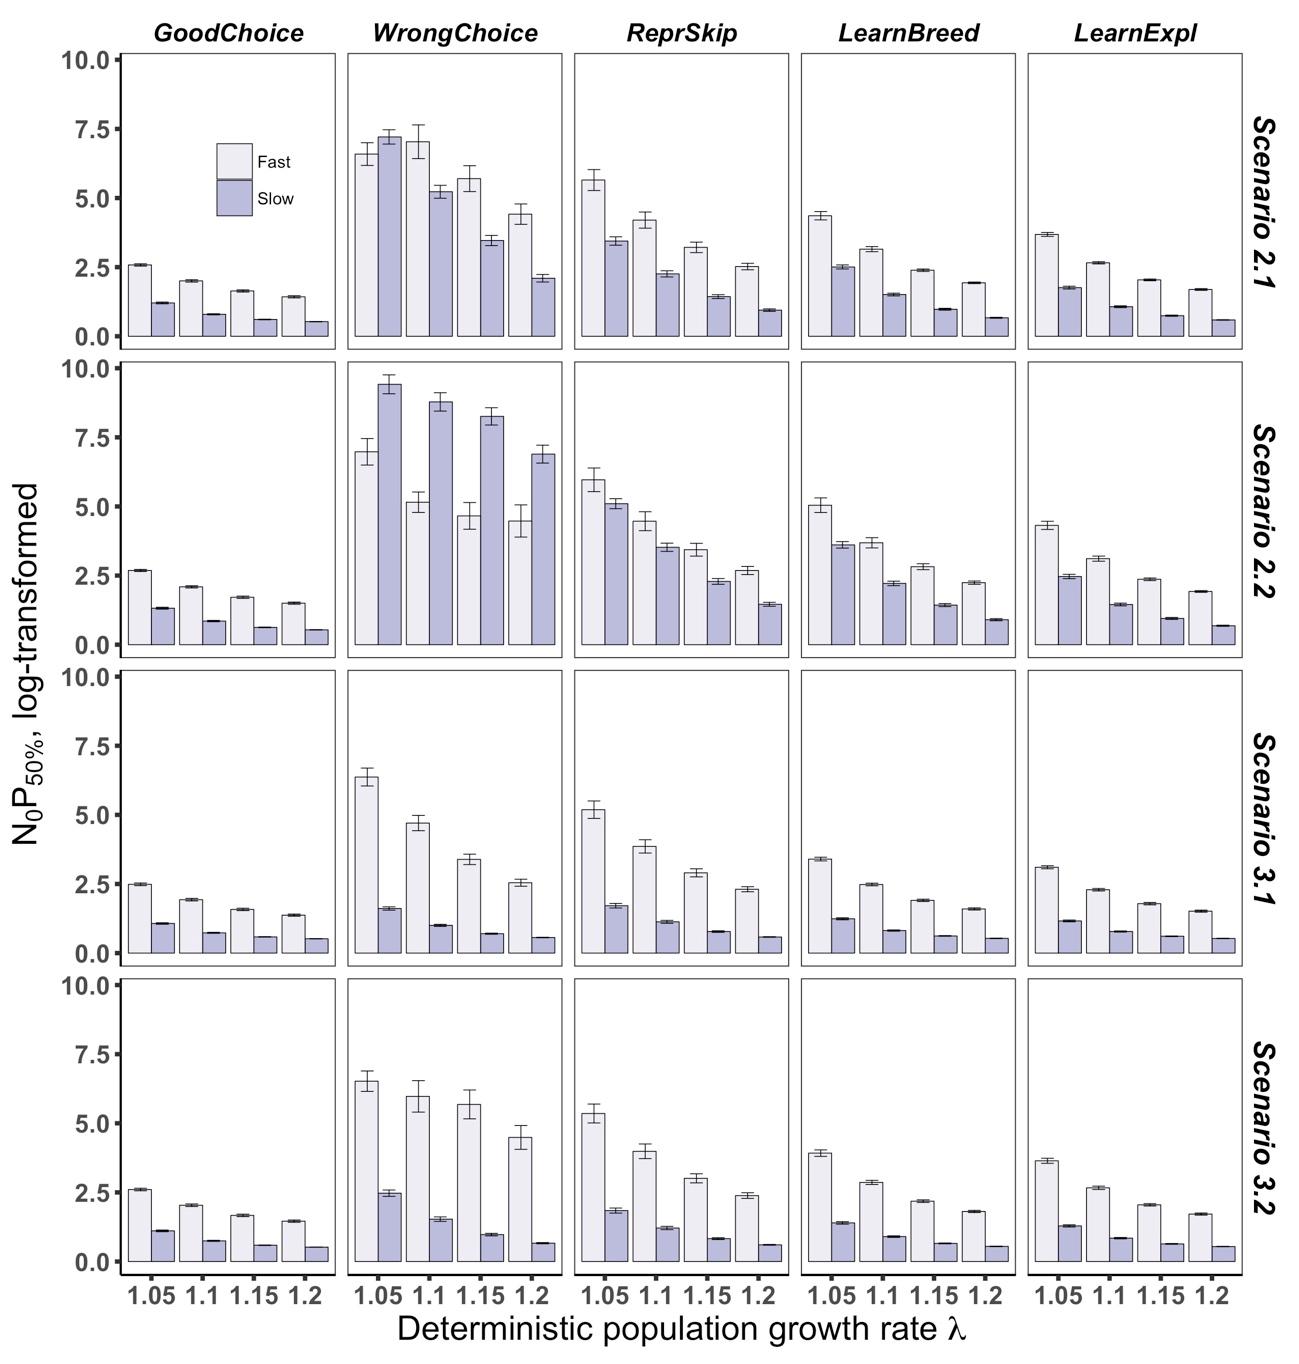
\includegraphics[width=\textwidth]{./Figures/Appendix3_2/Fig_4.jpg}
\caption[Effects on $N_{0}P_{50\%}$ with strong behavioural responses]{
Effects of behavioural responses on population persistence in novel
environments as a function of the position of the animal along the fast-slow
continuum. Population persistence is estimated as $N_{0}P_{50\%}$ and
behavioural responses are strong. The position of the animal along the fast-slow
continuum is assessed as the relative sensitivity (i.e. elasticity) of
population growth to changes in fecundity, with slow-lived strategies exhibiting
low elasticities and fast-lived strategies exhibiting high elasticities. For
details on abbreviation, see figure \ref{fig:fig3.1}.}
\label{fig:figApp3.2.4}
\end{figure}

\begin{figure}
\centering
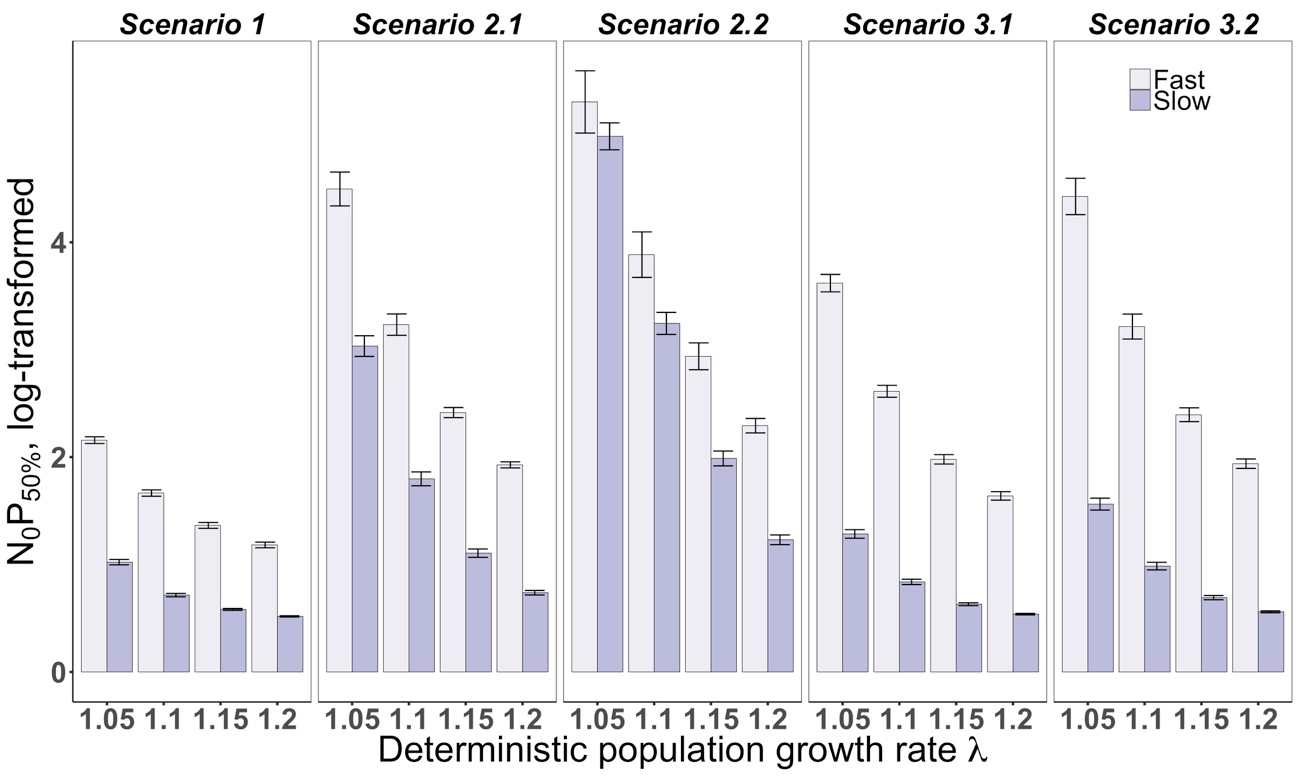
\includegraphics[width=\textwidth]{./Figures/Appendix3_2/Fig_5.jpg}
\caption[Effects on $N_{0}P_{50\%}$ with neutral behaviour]{
Population persistence in novel environments as a function of the
position of the animal along the fast-slow continuum for different scenarios and
neutral behaviour. Population persistence is estimated as $N_{0}P_{50\%}$.}
\label{fig:figApp3.2.5}
\end{figure}

\begin{figure}
\centering
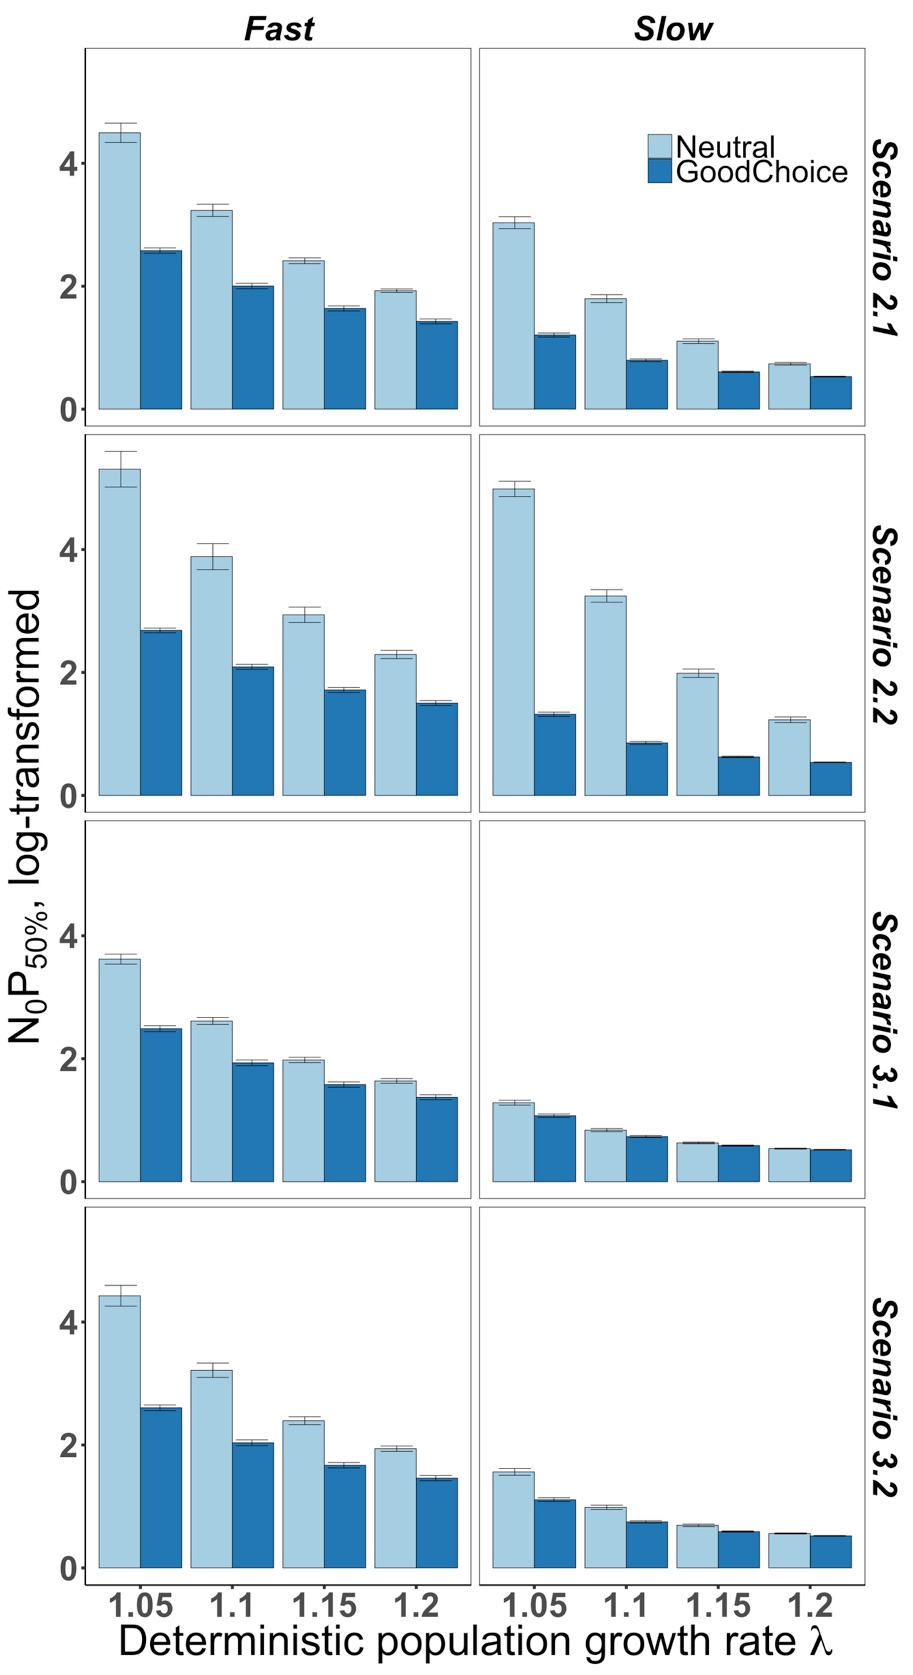
\includegraphics[height=.75\textheight]{./Figures/Appendix3_2/Fig_6.jpg}
\caption[Effects of \textit{GoodChoice} on $N_{0}P_{50\%}$]{
Influence of habitat matching choice on population persistence in novel
environments as a function of the position of the species along the fast-slow
continuum. Benefits and costs of the behaviour under different environmental
scenarios are reflected in differences in $N_{0}P_{50\%}$ between simulations
where individuals’ behaviour is either considered neutral or to reflect an
innate preference for the high-quality habitat.}
\label{fig:figApp3.2.6}
\end{figure}

\begin{figure}
\centering
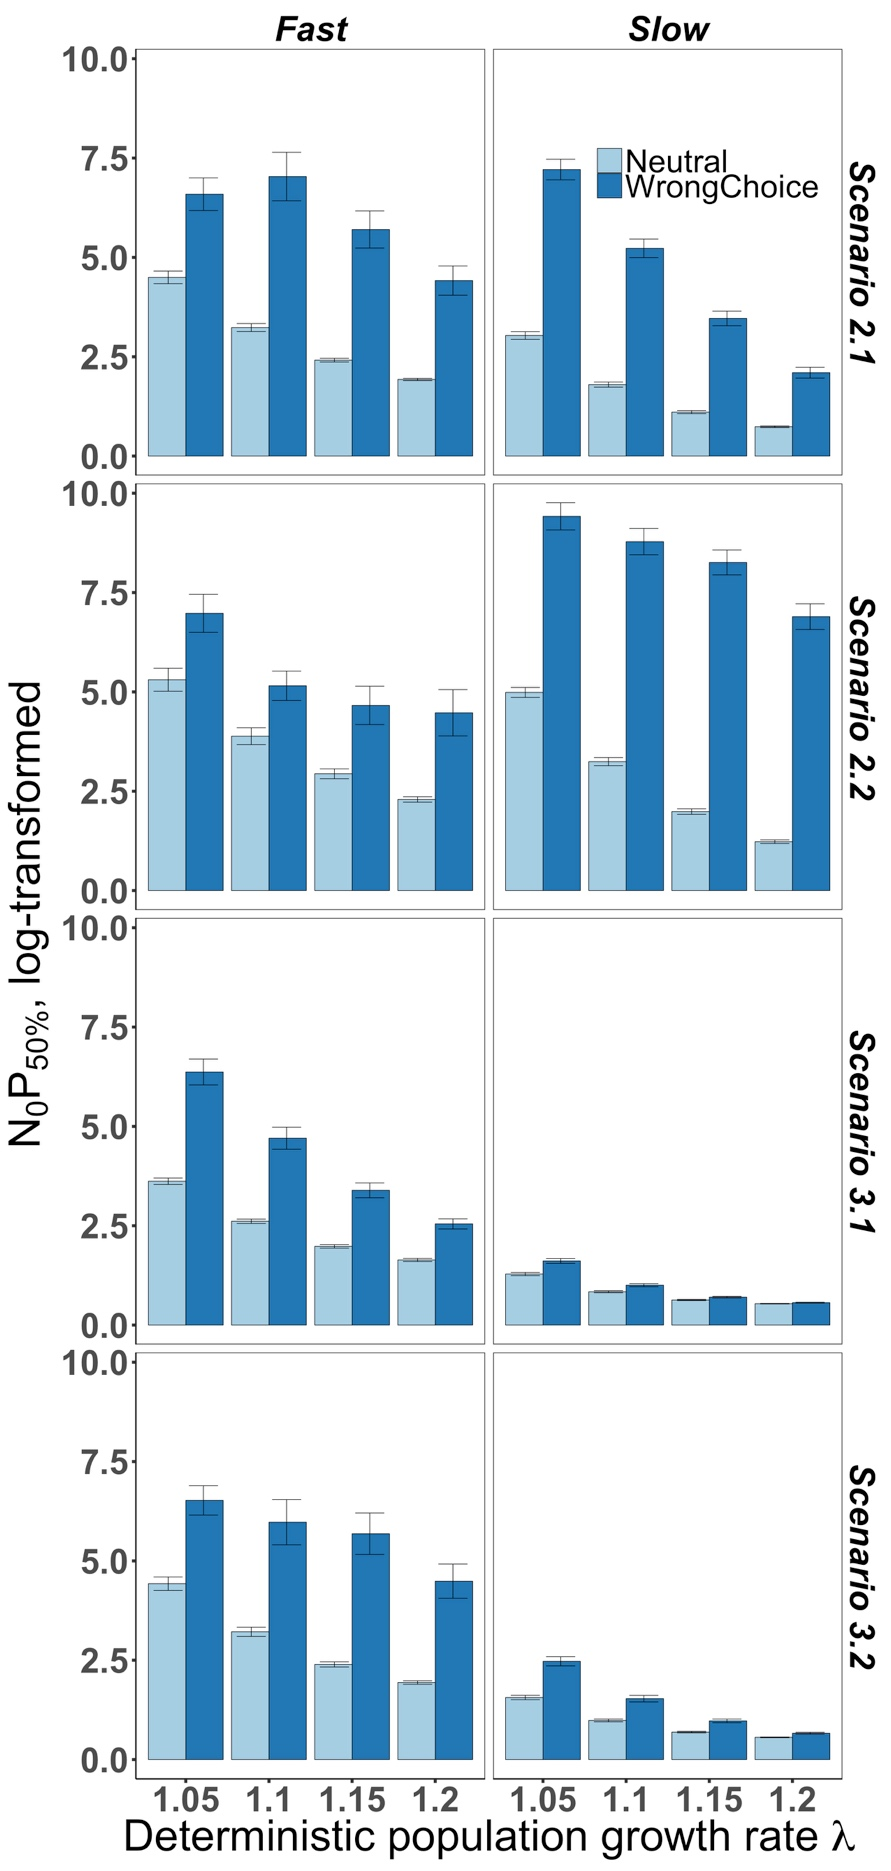
\includegraphics[height=.75\textheight]{./Figures/Appendix3_2/Fig_7.jpg}
\caption[Effects of \textit{WrongChoice} on $N_{0}P_{50\%}$]{
Influence of an inappropriate habitat matching choice on population persistence
in novel environments as a function of the position of the species along the
fast-slow continuum. Benefits and costs of the behaviour under different
environmental scenarios are reflected in differences in $N_{0}P_{50\%}$ between
simulations where individuals’ behaviour is either considered neutral or to
reflect an innate preference for the low-quality habitat.}
\label{fig:figApp3.2.7}
\end{figure}

\begin{figure}
\centering
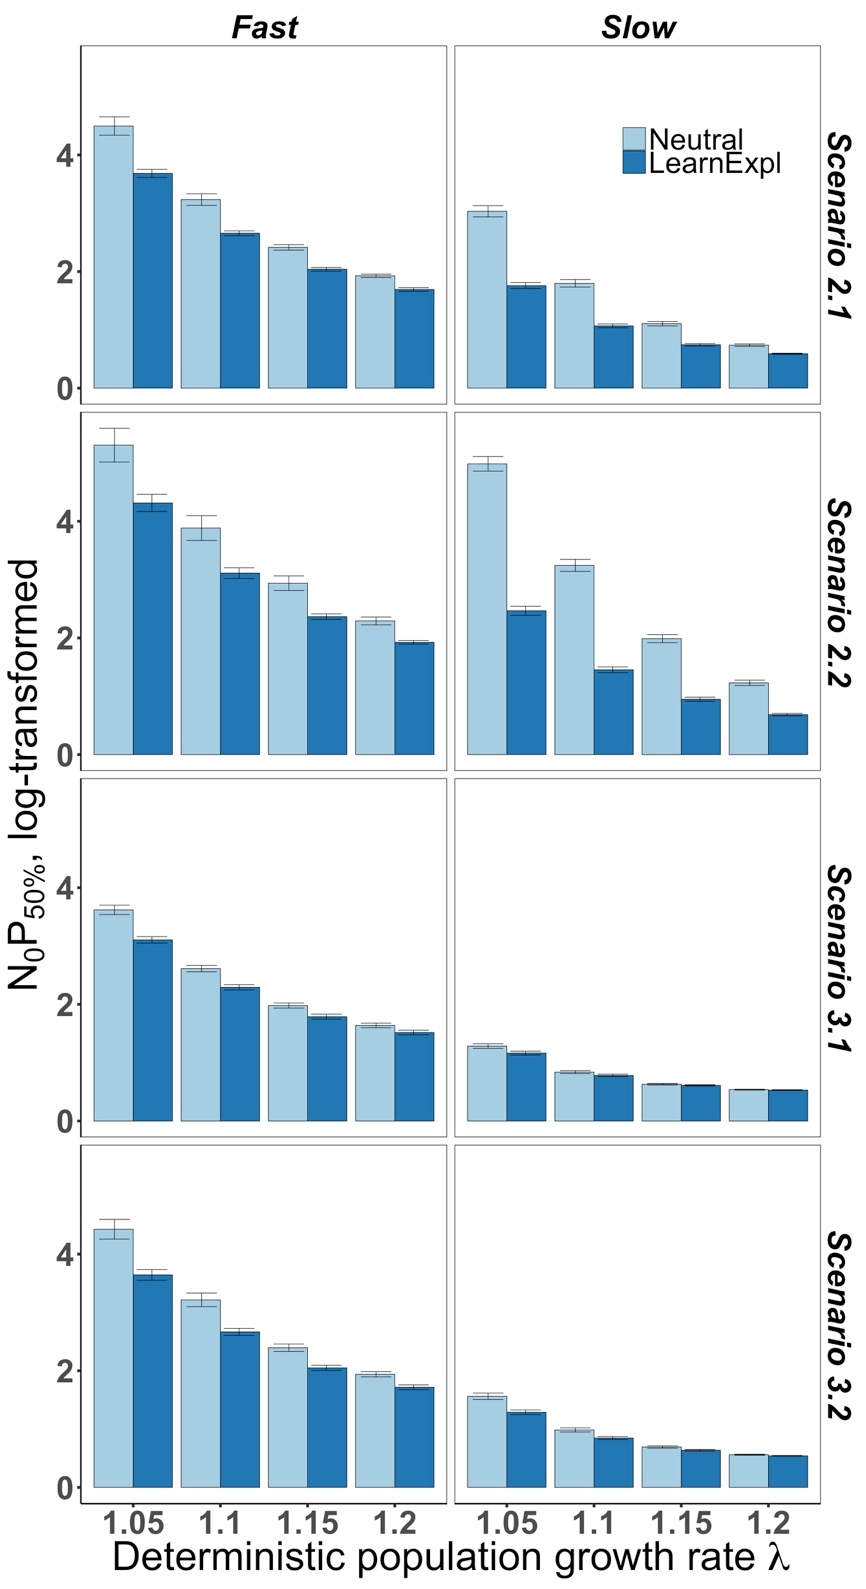
\includegraphics[height=.75\textheight]{./Figures/Appendix3_2/Fig_8.jpg}
\caption[Effects of \textit{LearnExpl} on $N_{0}P_{50\%}$]{
Influence of learning through exploration on population persistence in novel
environments as a function of the position of the species along the fast-slow
continuum. Benefits and costs of the behaviour under different environmental
scenarios are reflected in differences in $N_{0}P_{50\%}$ between simulations
where individuals show (\emph{LearnExpl}) or do not show (\emph{Neutral}) a
decreased preference for the low-quality habitat after exploring any of the two
habitats.}
\label{fig:figApp3.2.8}
\end{figure}

\begin{figure}
\centering
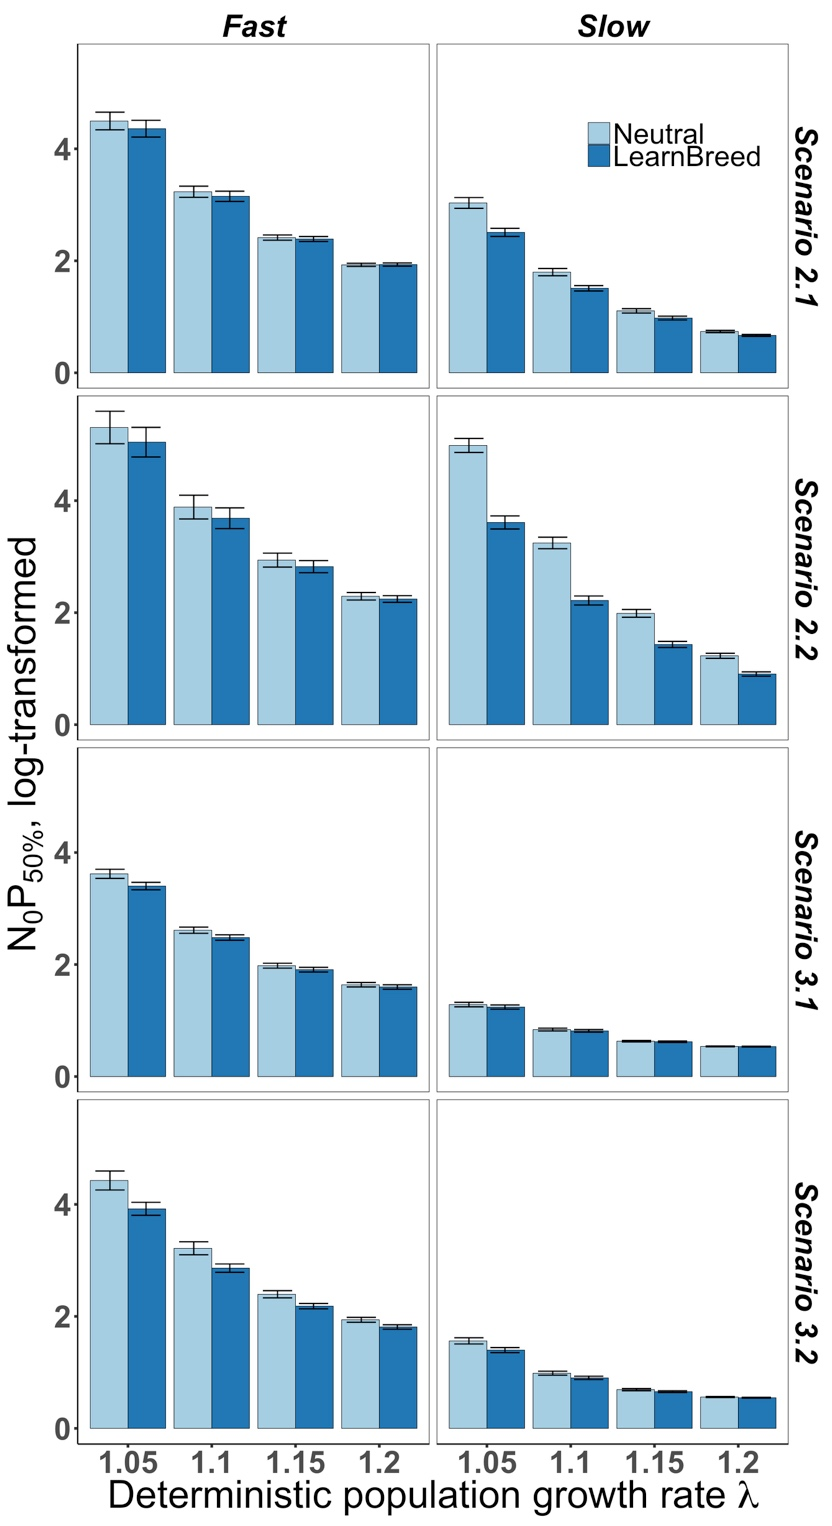
\includegraphics[height=.75\textheight]{./Figures/Appendix3_2/Fig_9.jpg}
\caption[Effects of \textit{LearnBreed} on $N_{0}P_{50\%}$]{
Influence of learning from a breeding experience on population persistence in
novel environments as a function of the position of the species along the
fast-slow continuum. Benefits and costs of the behaviour under different
environmental scenarios are reflected in differences in $N_{0}P_{50\%}$ between
simulations where individuals’ decision about changing habitat depends
(\emph{LearnBreed}) or not (\emph{Neutral}) on the success of the past breeding
attempt.}
\label{fig:figApp3.2.9}
\end{figure}

\begin{figure}
\centering
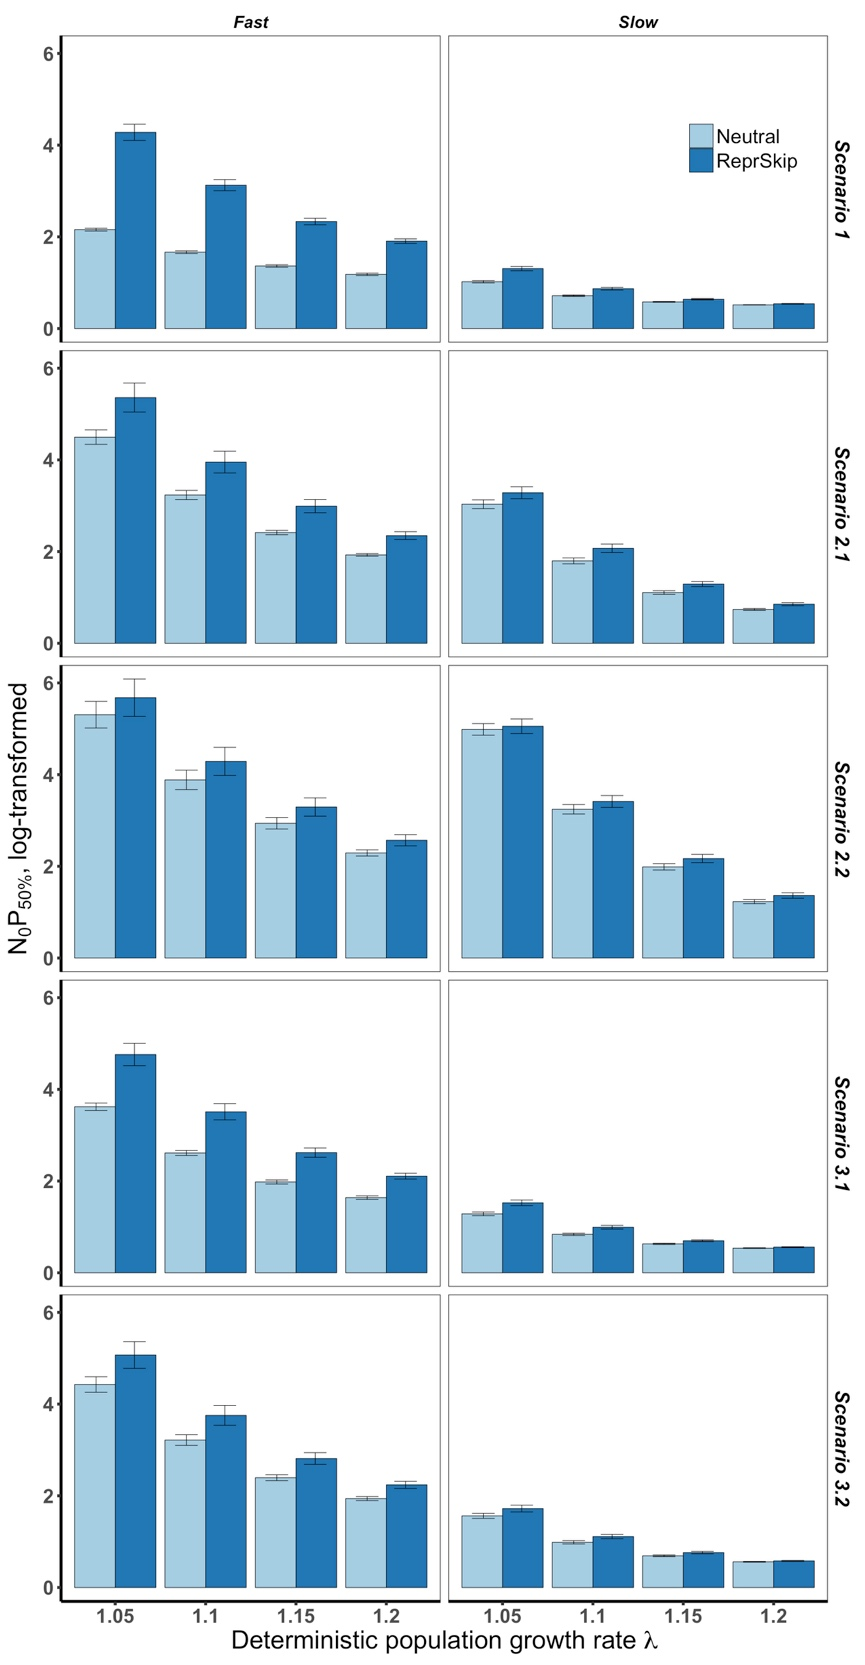
\includegraphics[height=.75\textheight]{./Figures/Appendix3_2/Fig_10.jpg}
\caption[Effects of \textit{ReprSkip} on $N_{0}P_{50\%}$]{
Influence of a reproductive skip on population persistence in novel environments
as a function of the position of the species along the fast-slow continuum.
Benefits and costs of the behaviour under different environmental scenarios are
reflected in differences in $N_{0}P_{50\%}$ between simulations where
individuals either have the option (\emph{ReprSkip}) or not (\{emph{Neutral}) to
skip a reproductive event.}
\label{fig:figApp3.2.10}
\end{figure}

\begin{figure}
\centering
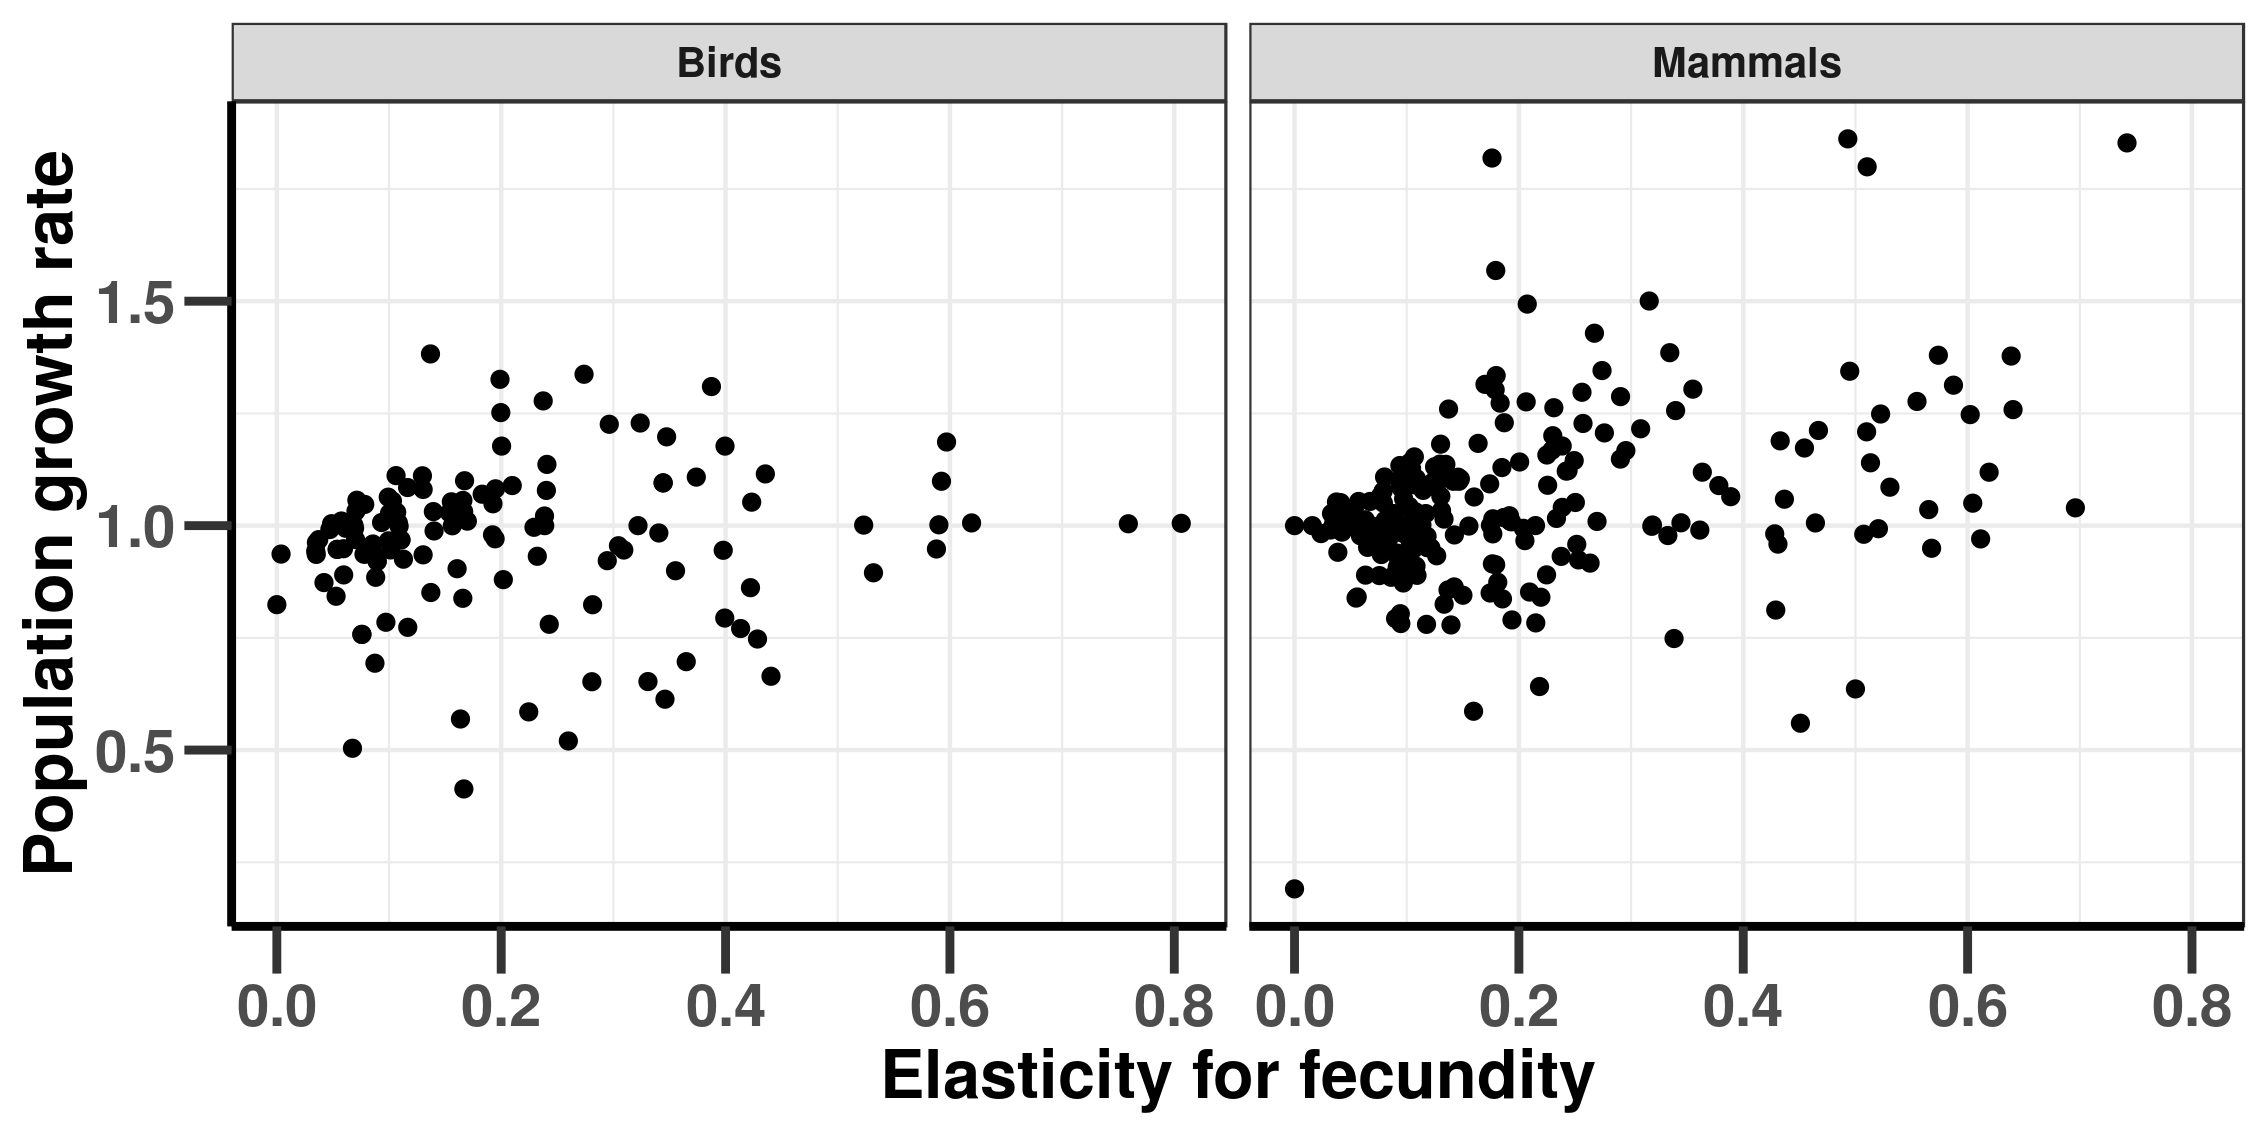
\includegraphics[width=\textwidth]{./Figures/Appendix3_2/Fig_11.png}
\caption[Fast-slow continuum and $\lambda$]{
Relationship between the fast-slow continuum and population grow rate
($\lambda$) in wild populations of birds and mammals suggesting that population
growth rate is not higher for fast-lived strategies than for slow-lived
strategies. Data come from COMADRE \citep{Salguero-Gomez2016}. The fast-slow
continuum is defined as the elasticity of population growth to changes in net
fecundity, based on demographic analysis using the popbio R-package
\cite{Stubben2007}.}
\label{fig:figApp3.2.11}
\end{figure}
